
\section{Versuchsdurchführung}

\subsection{ Allgemeiner Versuchsaufbau}

In diesem Termin werden folgende Geräte verwendet:
%
\begin{itemize}
    \item  Digitaloszilloskop Rigol MSO1074Z
    \item einstellbarer Funktionsgenerator Tektronix AFG1022
    \item einstellbare Spannungsquelle Rigol DP832
    \item USB-Oszilloskop, einstellbare Spannungsquelle Analog Discovery 2
\end{itemize}

\subsection{Der Phasenschieberoszillator}
%
In diesem Teilversuch werden folgende Bauteile verwendet:

\begin{itemize}
    \item Operationsverstärker TL072
    \item Ohmsche Widerstände mit $R_1=R_2=R_3=\SI{680}{\ohm}, R_4=\SI{56}{\kilo\ohm}, R_5=\SI{120}{\ohm}$
    \item Kondensator mit $C_1=C_2=C_3=\SI{100}{\nano\farad}$
\end{itemize}

Zunächst wird es ein passives Hochpassfilter dritter Ordnung aufgebaut. Drei Kondensatoren $C_1=C_2=C_3=\SI{100}{\nano\farad}$ werden in der Reihe geschaltet.Wie in Abbildung \ref{fig:passives_Hochpass} dargestellt, wird jeweils ein Ende der Widerstände $R_1=R_2=R_3=\SI{680}{\ohm}$ mit der Masse verbunden, während das andere Ende mit dem entsprechenden Kondensator verbunden ist.  \\
%korrigiert
  \begin{figure}[H]
  \centering
\begin{circuitikz}

%\begin{tikzpicture}[european,thick]
% First Stage
\draw (0,-1) node[ocirc]{} to[short] ++(3,0);
\draw (0,2) node[ocirc]{} to[C,a=\SI{100}{\nano\farad},l=$C_1$] ++(2,0) coordinate(a);
\draw (a) to[short] ++(1,0);
\draw (a) to[R,a=\SI{680}{\ohm},l=$R_1$,*-*] ++(0,-3);

% Second Stage
\draw (3,-1) to[short] ++(3,0);
\draw (3,2) to[C,a=\SI{100}{\nano\farad},l=$C_2$] ++(2,0) coordinate(b);
\draw (b) to[short] ++(1,0);
\draw (b) to[R,a=\SI{680}{\ohm},l=$R_2$,*-*] ++(0,-3) -- (5,-1.5) node[ground]{};;

% Third Stage
\draw (6,-1) to[short] ++(3,0);
\draw (6,2) to[C,a=\SI{100}{\nano\farad},l=$C_3$] ++(2,0) coordinate(c)  ;
\draw (8,2) --(10,2) node[ocirc]{};
\draw (c) to[R,a=\SI{680}{\ohm},l=$R_3$ ,*-*] (8, -1) -- (10, -1) node[ocirc]{};

% Voltage labels

\draw [-latex] ([yshift=-2mm] 0,2)--(0,-0.9) node[midway,left] {$U_e$} ;  
\draw [-latex] ([yshift=-2mm] 10,2)--(10,-0.9) node[midway,left] {$U_a$};  

%\end{tikzpicture}
\end{circuitikz}
\caption{passives Hochpassfilter 3.Ordnung}
\label{fig:passives_Hochpass}
\end{figure}

Dann wird ein invertierender Verstärker aufgebaut. Zwischen dem Eingangssignal und dem invertierenden Eingangs des OPVs befindet sich der Widerstand $R_5=\SI{120}{\ohm}$. Der Widerstand $R_4=\SI{56}{\kilo\ohm}$ wird zwischen dem invertierenden Eingang und des Ausgang des OPVs angeschlossen.
%
  \begin{figure}[H]
  \centering
\begin{circuitikz}[european]
    \ctikzset{bipoles/length=1cm}
    
    \draw
    (0,0) node[op amp] (opamp) {};
    
    \draw (opamp.-) to[R, european resistor, l=$R_5$,a=\SI{120}{\ohm}] (-2.5, 0.35) -- (-3, 0.35) node[ocirc]{};
    
    \draw [-latex] ([yshift=-2mm] -3,0.35)--(-3,-1.35) node[midway,left] {$U_e$} ; 
   
 % Zeichne C   
    \draw (opamp.-) to[short,*-] ++(0,1.25) coordinate (leftD) 
    to[R, l=$R_4$,a=\SI{56}{\kilo\ohm}] (leftD -| opamp.out)  ;

    \draw [-latex] ([yshift=-2mm] 2,0)--(2,-1.35) node[midway,left] {$U_a$}; 
    
    \draw (2,-1.45) node[ocirc]{} to(2,-1.5) node[ground]{};
    \draw (-3,-1.45)node[ocirc]{}to(-3,-1.5) node[ground]{};

   \draw (opamp.out)--(2,0) node[ocirc]{};
 
   \draw (leftD -| opamp.out) --(1.5,1.55)  to[short,-*] (1.5,0);

    \draw (opamp.+) -- (-1,-0.35) to (-1,-1.5) node[ground]{};
  
\end{circuitikz}
\end{figure}

Danach wird der Ausgang des Hochpassfilters an den Eingang des invertierenden Verstärkers angeschlossen. Ebenfalls wird der Ausgang des invertierender Verstärkers mit dem Eingang des Hochpassfilters verbunden.

Die Abbildung \ref{fig:Steckbrett_Phasenschieberoszillator} zeigt, wie der Phasenschieberoszillator aus einem passiven Hochpassfilter und aus einem invertierender Verstärker auf einem Steckbrett realisiert werden kann.

\begin{figure}[H]
  \centering
  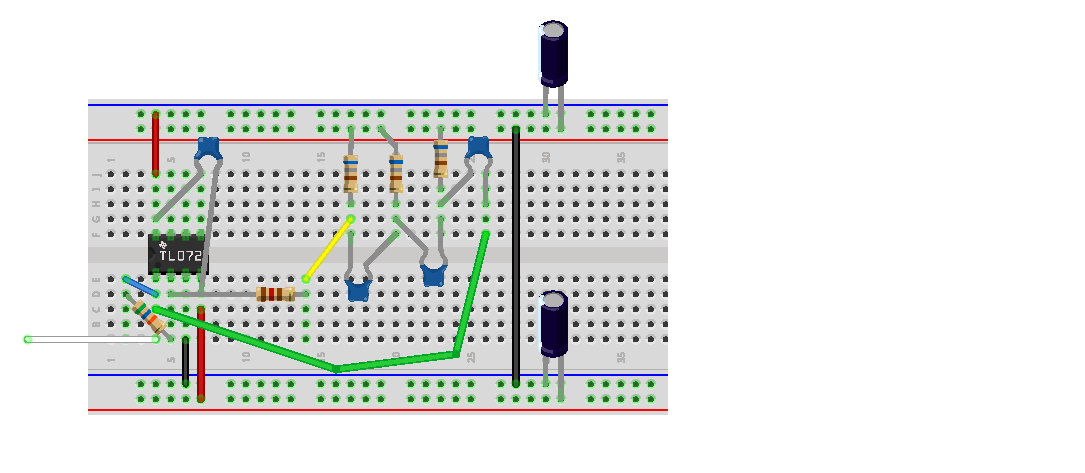
\includegraphics[width=0.7\linewidth]{Elektronik-Laborprotokoll_Filter/Abbildungen/Steckbrett_Bilder_Fritzing/Steckbrett_Aufgabe_1.pdf}
  \caption{Phasenschieberoszillator(Steckbrett)}
  \label{fig:Steckbrett_Phasenschieberoszillator}
\end{figure}
%
\subsection{NE555}
%
In diesem Teilversuch werden folgende Bauteile verwendet:
%
\begin{itemize}
    \item NE555 Oszillator
    \item Ohmsche Widerstände $R_1=\SI{680}{\ohm},R_2=\SI{2,7}{\kilo \ohm}$
    \item Potentiometer
    \item 2 x Dioden
    \item Kondensatoren mit $C_1=C_2=C_3=\SI{100}{\nano\farad}$
\end{itemize}

\subsubsection{NE555 Oszillator}
Als erstes wird der NE555 im astabilen Modus betrieben. 

\begin{figure}[H]
  \centering
  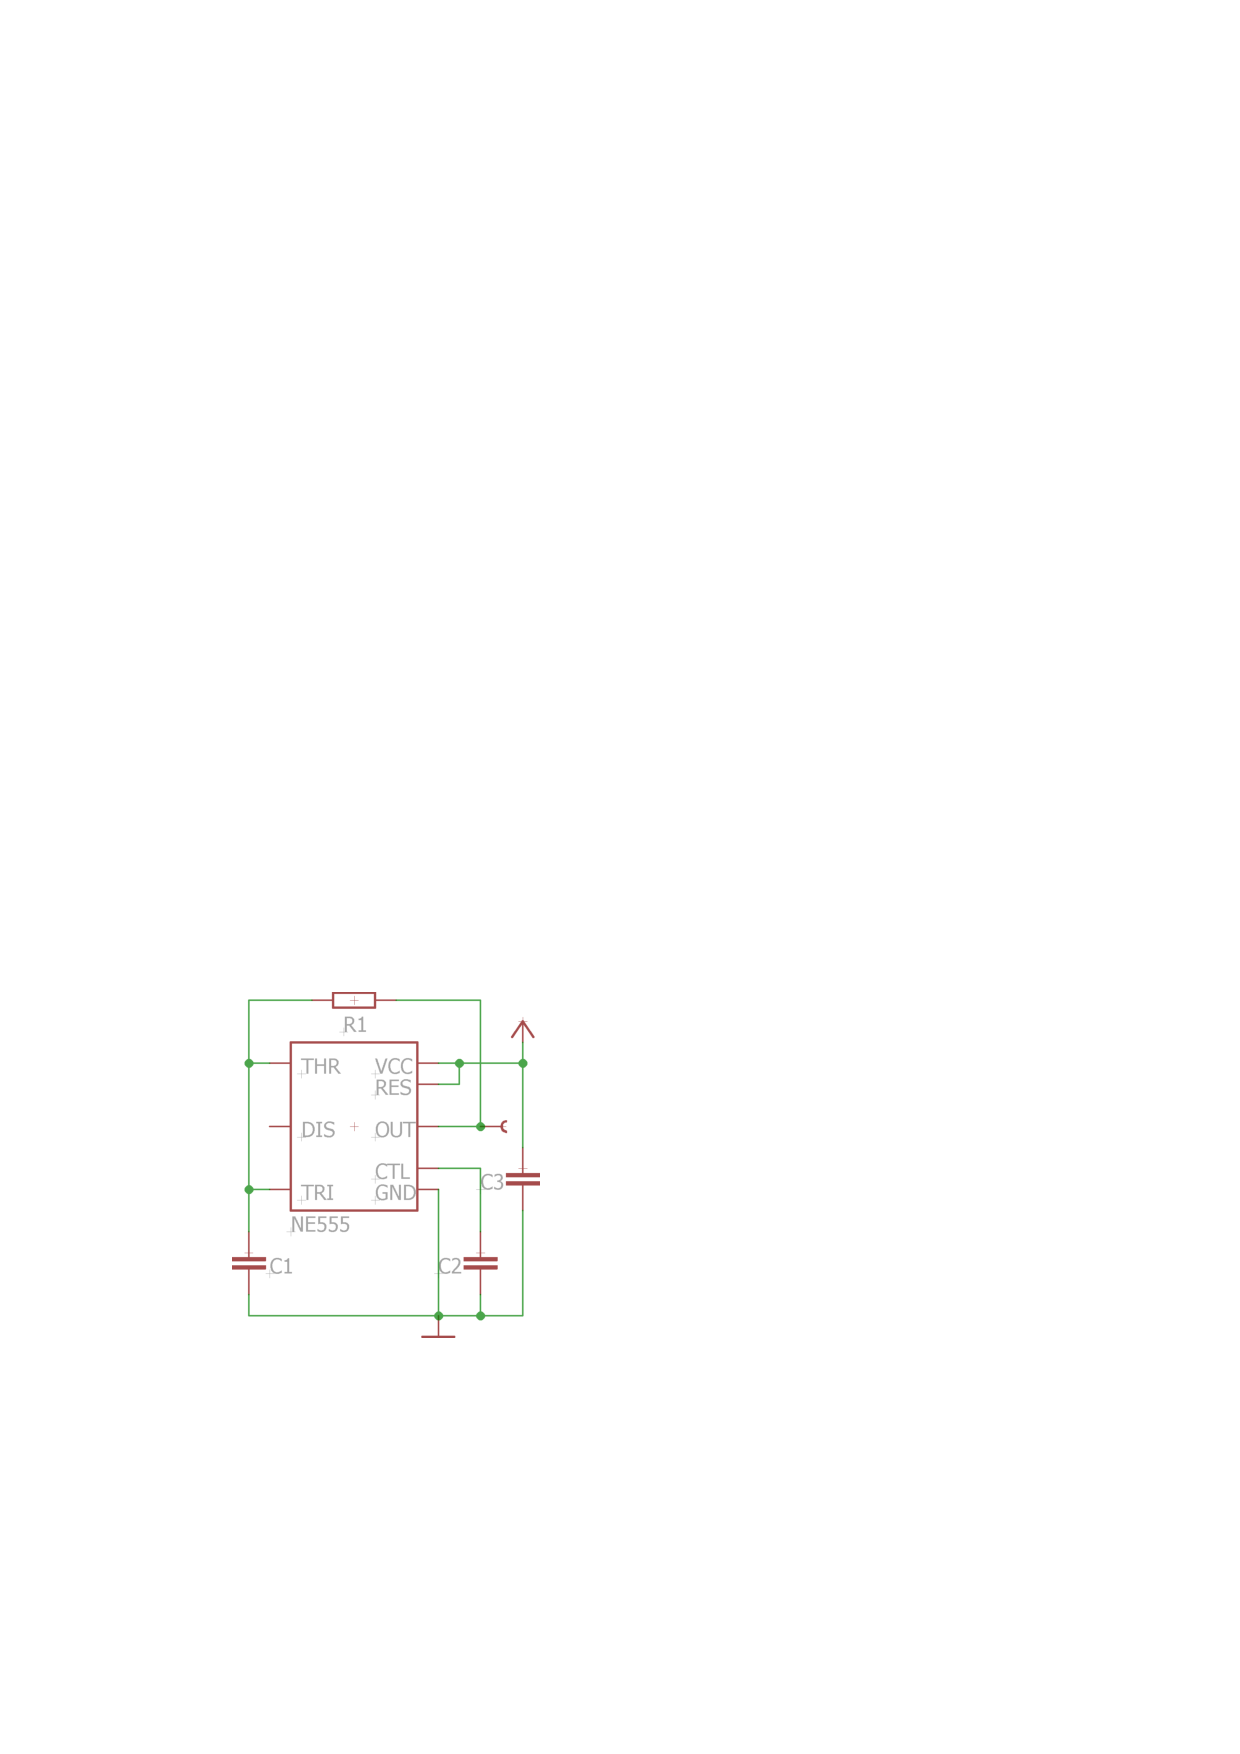
\includegraphics[width=0.5\linewidth]{Elektronik-Laborprotokoll_Filter/Abbildungen/Schaltungen_Skript/Schaltung_NE555_astabile_Kippstufe.pdf}
  \caption{50\% Tastgrad (Schaltung)\cite{Skript}}
  \label{fig:astabiler_Modus}
\end{figure}


Die Schaltung wird so dimensioniert (\ref{fig:Steckbrett_NE555_1}), dass die Oszillationsfrequenz \SI{10}{\kilo\hertz} und der von 50\% beträgt. Neben den drei Kondensatoren $C_1=C_2=C_3=\SI{100}{\nano\farad}$ wird der Widerstand  $R_1=\SI{680}{\ohm}$ in der Schaltung verwendet.

%GELÖST
\begin{figure}[H]
  \centering
  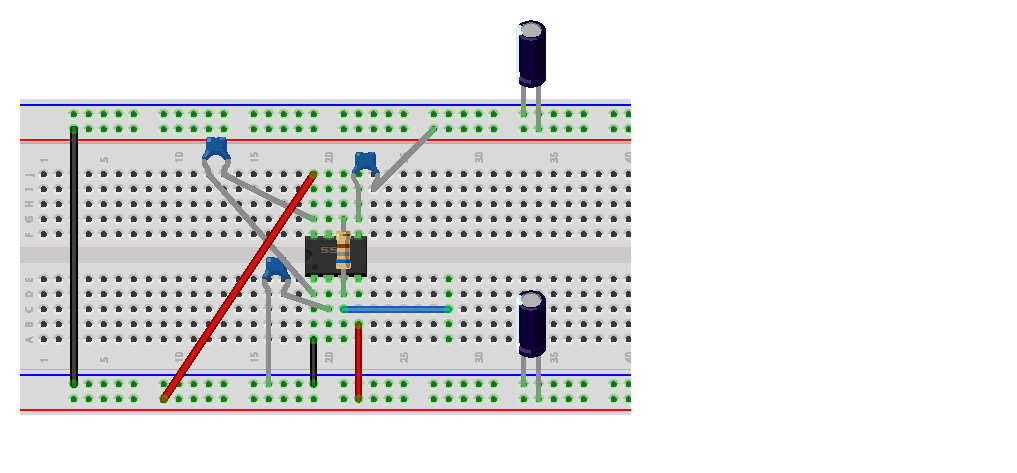
\includegraphics[width=0.5\linewidth]{Elektronik-Laborprotokoll_Filter/Abbildungen/Steckbrett_Bilder_Fritzing/Steckbrett_Aufgabe_2.1_NE555_1_bb.pdf}
  \caption{50\% Tastgrad (Steckbrett)}
  \label{fig:Steckbrett_NE555_1}
\end{figure}

Die Schaltung wird so erweitert (\ref{fig:astabiler_Modus_einstellbar}), dass der Tastgrad einstellbar ist.

\begin{figure}[H]
  \centering
  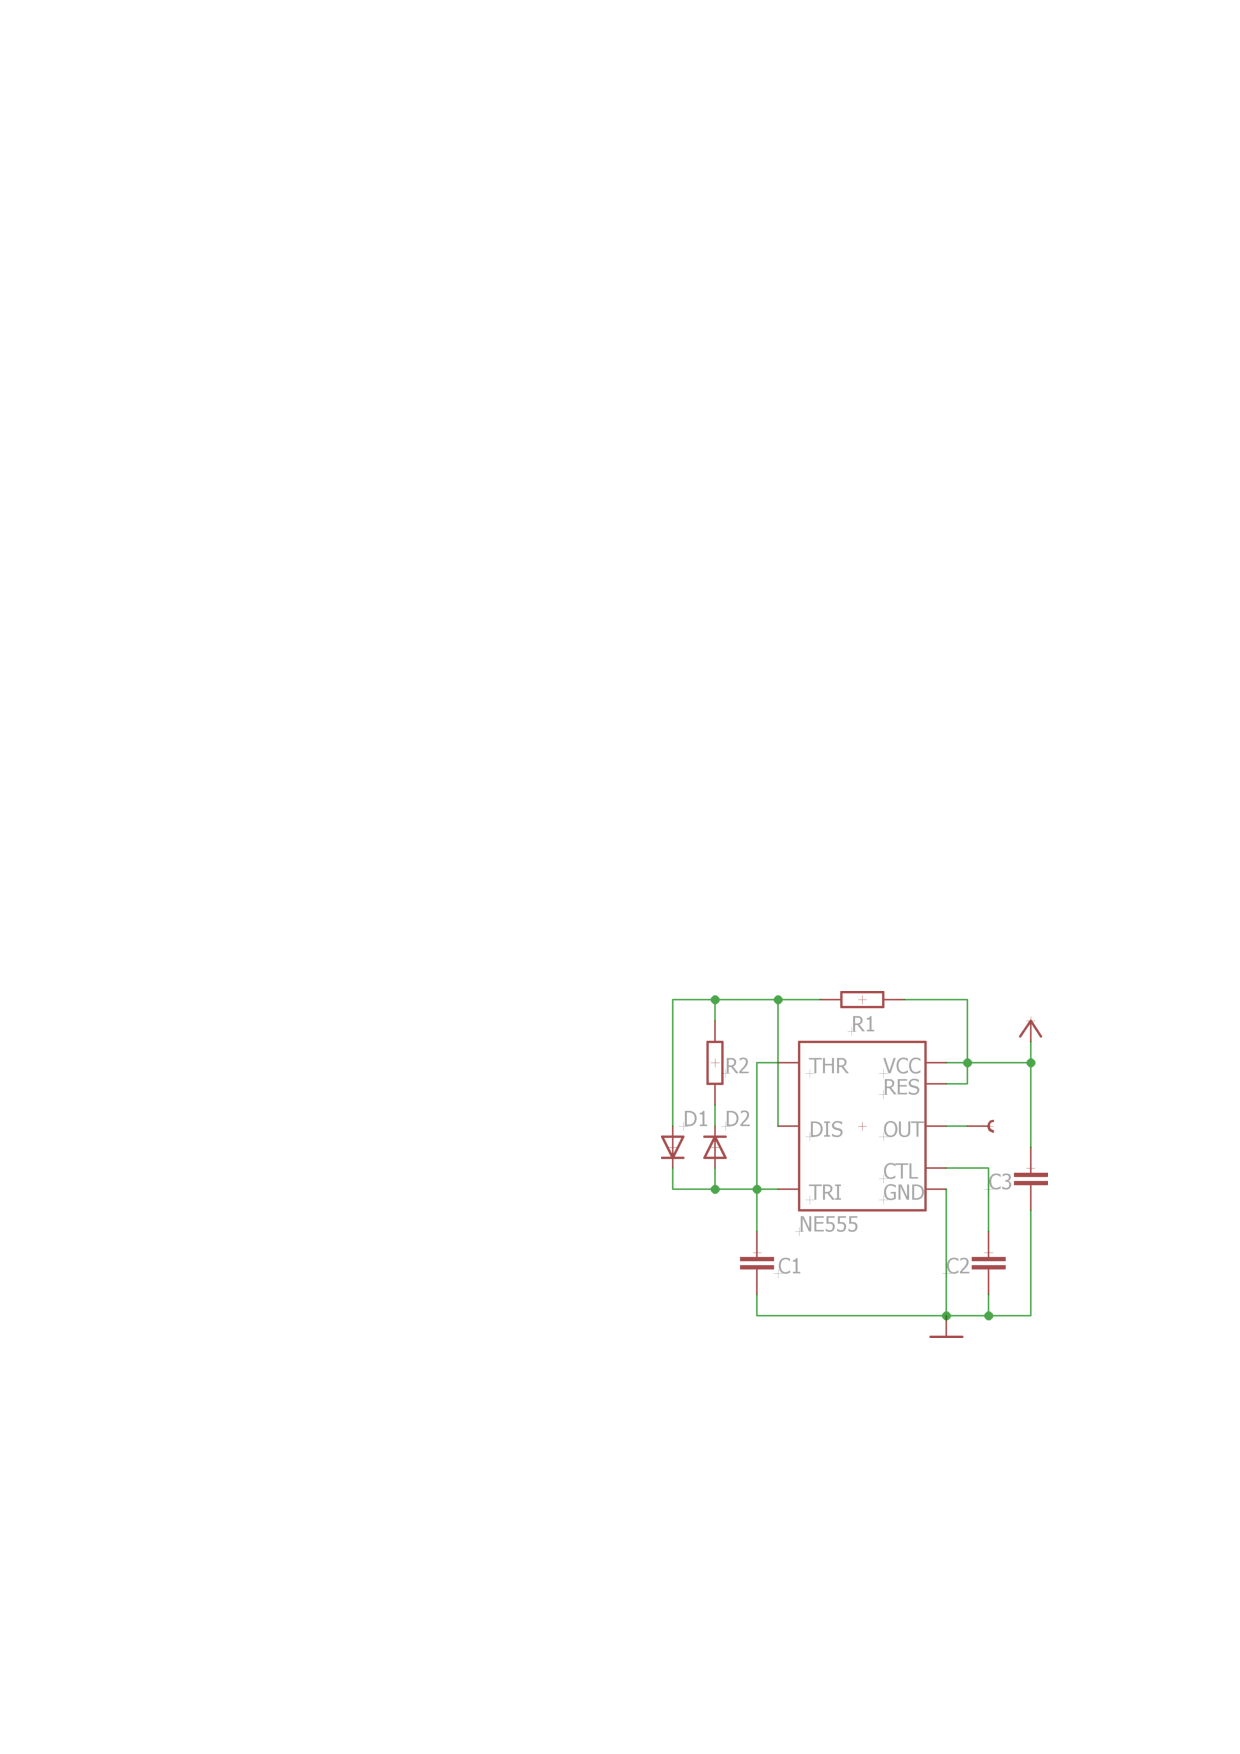
\includegraphics[width=0.5\linewidth]{Elektronik-Laborprotokoll_Filter/Abbildungen/Schaltungen_Skript/Schaltung_NE555_einstellbarer Tastgrad.pdf}
  \caption{einstellbarer Tastgrad (Schaltung)\cite{Skript}}
  \label{fig:astabiler_Modus_einstellbar}
\end{figure}

Die Widerstände $R_1$ und $R_2$ werden mit einem Potentiometer ersetzt (\ref{fig:Steckbrett_NE555_2}), um die Einstellung des gewünschten Tastgrades zu vereinfachen.

\begin{figure}[H]
  \centering
  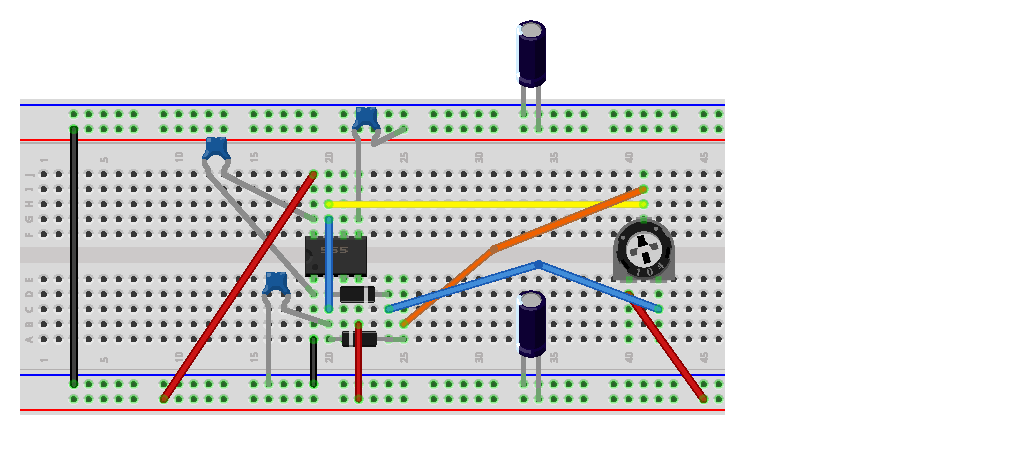
\includegraphics[width=0.5\linewidth]{Elektronik-Laborprotokoll_Filter/Abbildungen/Steckbrett_Bilder_Fritzing/Steckbrett_Aufgabe_2.2_NE555_pm.pdf}
  \caption{einstellbarer Tastgrad (Steckbrett)}
  \label{fig:Steckbrett_NE555_2}
\end{figure}

\subsubsection{Monoflop}

\begin{figure}[H]
  \centering
  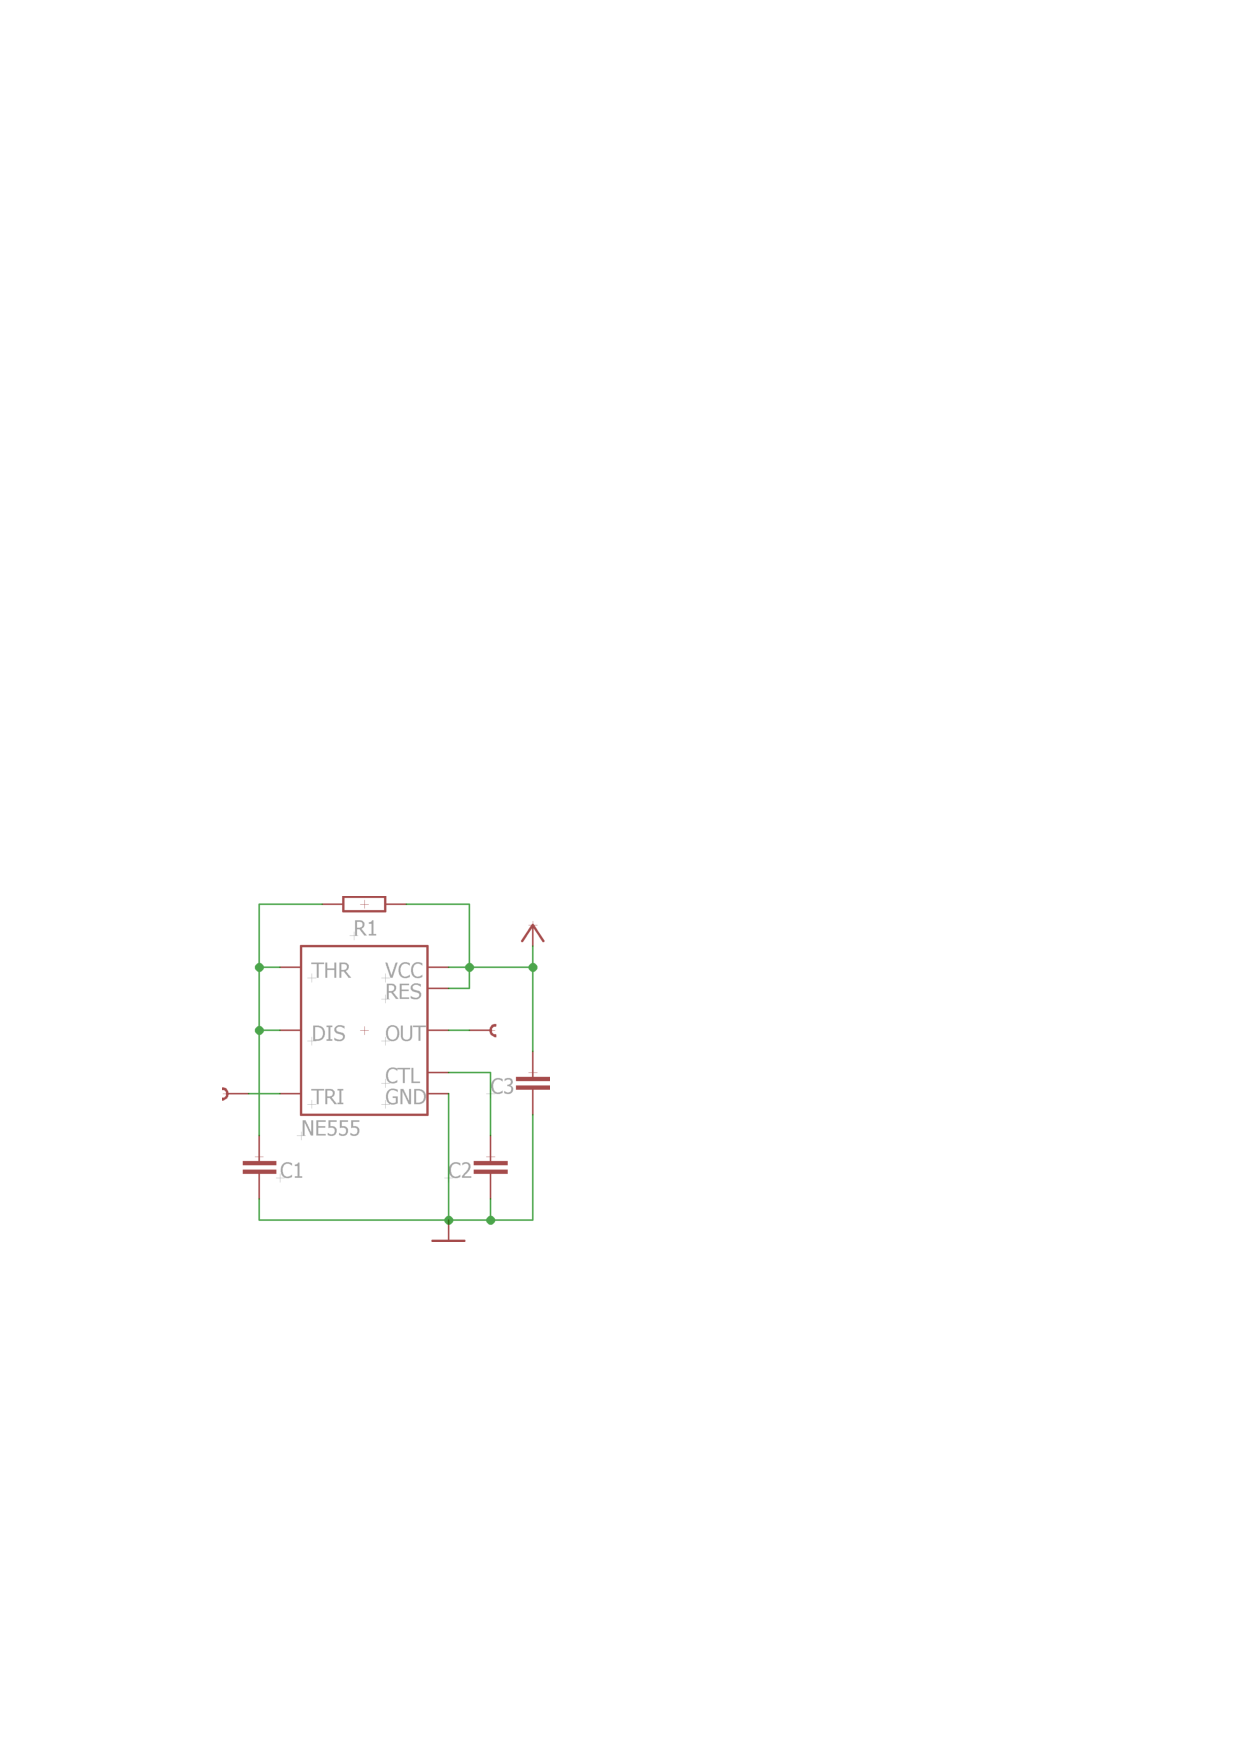
\includegraphics[width=0.5\linewidth]{Elektronik-Laborprotokoll_Filter/Abbildungen/Schaltungen_Skript/Schaltung_NE555_Monoflop.pdf}
  \caption{Monoflop (Schaltung)\cite{Skript}}
  \label{fig:Monoflop_Schaltung}
\end{figure}
Danach wird ein Monoflop mit einer Zeitkonstante von $\tau=\SI{100}{\micro\second}$ aufgebaut (\ref{fig:Steckbrett_NE555_3}):

\begin{figure}[H]
  \centering
  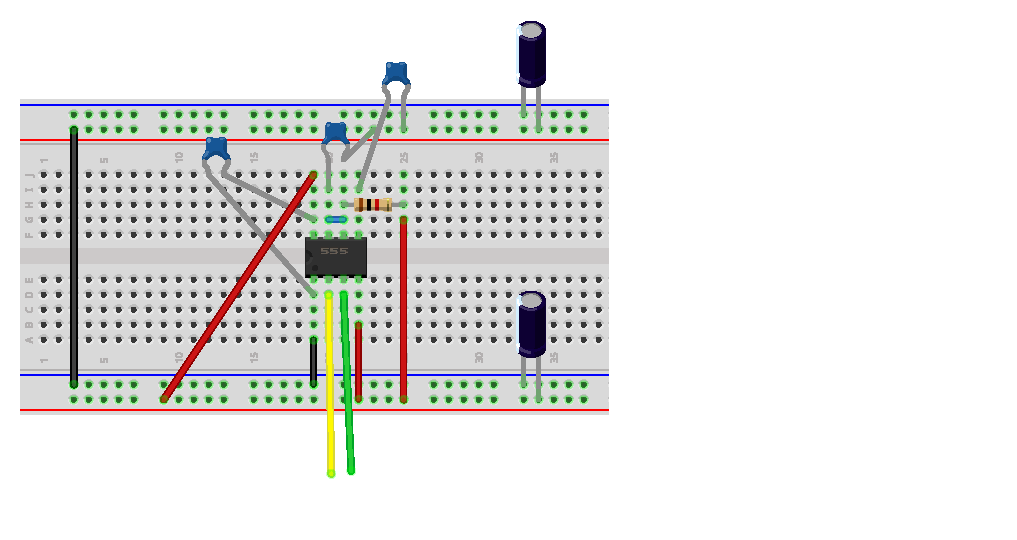
\includegraphics[width=0.5\linewidth]{Elektronik-Laborprotokoll_Filter/Abbildungen/Steckbrett_Bilder_Fritzing/Steckbrett_Aufgabe_2.3_NE555__monoflop.pdf}
  \caption{Monoflop (Steckbrett)}
  \label{fig:Steckbrett_NE555_3}
\end{figure}






%Mithilfe der Formel ..
%erhält man R=720 Ohm , haben wir aber 680

%NE555 wurde verwendet
% gebaut
%Kondensatoren imemr 100nF
%R1 berechnet 

%%%%%%%%\begin{figure}[H]
%%%%%%%%%%  \centering
%%%%%%%%\%begin{circuitikz}[european,scale=1, transform shape]
    %%%%% Draw resistors
  %%%%%%%%%%%%  \draw (0,0) to[R, l=$R_1$] (0,2); % First resistor R1
  %%%%%%%%%%%  \draw (1,0) to[R, l=$R_2$] (1,2); % Second resistor R%2
%%%%%%%%%%%%%    \draw (3,0) to[R, l=$R_3$] (3,2); % Third resistor R%%3
 %%%%%%%%%%%%%%   \draw (4,0) to[R, l=$R_4$] (4,2); % Fourth resistor R%4
  %%%%%%%%%%%%%%%  \draw (2,2) to[short] ++(0,1) node[vcc] {$V_{CC}$}%;
    %%%% Dra%w horizontal lines
  %%%%%%%%%%%%%%%  \draw (0,2) to[short] (4,2); % Top horizontal lin%e
   % 
    %%%%Draw capacitor
   %%%%%%%%%%%%%%%% \draw (0,0) to[short] (0,0)
%   to[C, l_%=$C$] (1,0); % Capacitor C
          %to[shor%t] (2,0); % Connect to lower part of the circuit

    %%%% Complete lower part of the circuit
    %\draw (3,0) to[C, l_=$C$] (4,0); % Bottom horizontal line
    
        %%%% Draw transistors
    %\draw (0,-3) node[npn,xscale=-1, anchor=E] (T1) {} % Transistor %%%T1
       %   (4,-3) node[npn, anchor=E] (T2) {}; % Transistor T2 %%%mirrored
 %%%%%%   \draw (0,0) to[short] (T1.C); 
  %%%%%%  \draw (3,0) to[short] (T1.B); 
  %%%%%%  \draw (1,0) to[short] (T2.B); 
%%%  %%  \draw (4,0) to[short] (T2.C); 
  % %%% \draw (T1.E) to[short] ++(0,-0.5) node[ground] {};
% %  % \draw (T2.E) to[short] ++(0,-0.5) node[ground] {};
%\en%d{circuitikz}
%\end{figure}
%In diesem Teilversuch wurde**** aufgebaut.


%Es wurden folgende Bauteile verwendet:
%
%\begin{itemize}
%    \item Operationsverstärker TL072
 %   \item Ohmsche Widerstände mit $R_1=\SI{10}{\kilo\ohm}$ und $R_2=\SI{1}{\mega\ohm}$  %Wie groß?
  %  \item Kondensator mit $C=\SI{100}{\nano\farad}$
%\end{itemize}

\subsection{Dreieck-Rechteck-Oszillator}

In diesem Teilversuch werden folgende Bauteile verwendet:

\begin{itemize}
    \item Operationsverstärker TL072
    \item Ohmsche Widerstände $R_1=\SI{10}{\kilo \ohm},R_2=\SI{22}{\kilo\ohm},R_3=\SI{2,7}{\kilo\ohm}$
    \item Kondensator $C=\SI{100}{\nano\farad}$
\end{itemize}

Erstens wird ein nicht invertierender Schmitt-Träger mit  $R_1=\SI{10}{\kilo \ohm}$ und $R_2=\SI{22}{\kilo\ohm}$ aufgebaut.

%korrigiert Schmitt-Träger
  \begin{figure}[H]
  \centering
  \begin{circuitikz}[european]

    \ctikzset{bipoles/length=1cm}
    
    \draw
    (0,0) node[op amp,yscale=-1] (opamp) {};
    
    \draw (opamp.+) to[R, european resistor, l=$R_1$] (-2, 0.35) -- (-3, 0.35) node[ocirc]{};
    
    \draw [-latex] ([yshift=-2mm] -3,0.35)--(-3,-1.35) node[midway,left] {$U_e$} ; 
   
  
    \draw (opamp.+) to[short,*-] ++(0,0.75) coordinate (leftD) to[short](leftD)
    to[R, european resistor, l=$R_2$] (leftD -| opamp.out) to [short,-*] (opamp.out) ;

    \draw [-latex] ([yshift=-2mm] opamp.out)--(0.85,-1.35) node[midway,left] {$U_a$}; 
    
    \draw (0.85,-1.45) node[ocirc]{} to(0.85,-1.5) node[ground]{};
    \draw (-3,-1.45)node[ocirc]{}to(-3,-1.5) node[ground]{};

   \draw (opamp.out)--(2,0) node[ocirc]{};
% Zeichne R2

    \draw (opamp.-) -- (-1,-0.35) to (-1,-1.5) node[ground]{};
    %\end{tikzpicture}
\end{circuitikz}
\end{figure}


Dann wird ein Integrator aufgeabaut:
 \begin{figure}[H]
  \centering
\begin{circuitikz}[european]
    \ctikzset{bipoles/length=1cm}
    
    \draw
    (0,0) node[op amp] (opamp) {};
    
    \draw (opamp.-) to[R, european resistor, l=$R_1$] (-2, 0.35) -- (-3, 0.35) node[ocirc]{};
    
    \draw [-latex] ([yshift=-2mm] -3,0.35)--(-3,-1.35) node[midway,left] {$U_e$} ; 
   
 % Zeichne C   
    \draw (opamp.-) to[short,*-] ++(0,0.75) coordinate (leftD) to[short,-*](leftD)
    to[C, l=$C$] (leftD -| opamp.out) to[short,-*](leftD -| opamp.out) ;

    \draw [-latex] ([yshift=-2mm] opamp.out)--(0.85,-1.35) node[midway,left] {$U_a$}; 
    
    \draw (0.85,-1.45) node[ocirc]{} to(0.85,-1.5) node[ground]{};
    \draw (-3,-1.45)node[ocirc]{}to(-3,-1.5) node[ground]{};

   \draw (opamp.out)--(2,0) node[ocirc]{};
% Zeichne R2
   \draw (leftD -| opamp.out) to[short,*-](leftD -| opamp.out) to ( opamp.out);

    \draw (opamp.+) -- (-1,-0.35) to (-1,-1.5) node[ground]{};

    
\end{circuitikz}
\end{figure}

Die Abbildung \ref{fig:Steckbrett_Phasenschieberoszillator} zeigt, wie der Dreieck-Rechteck-Oszillator aus einem nicht invertierenden Schmitt-Trigger und aus einem invertierenden Integrator auf einem Steckbrett realisiert werden kann.

\begin{figure}[H]
  \centering
  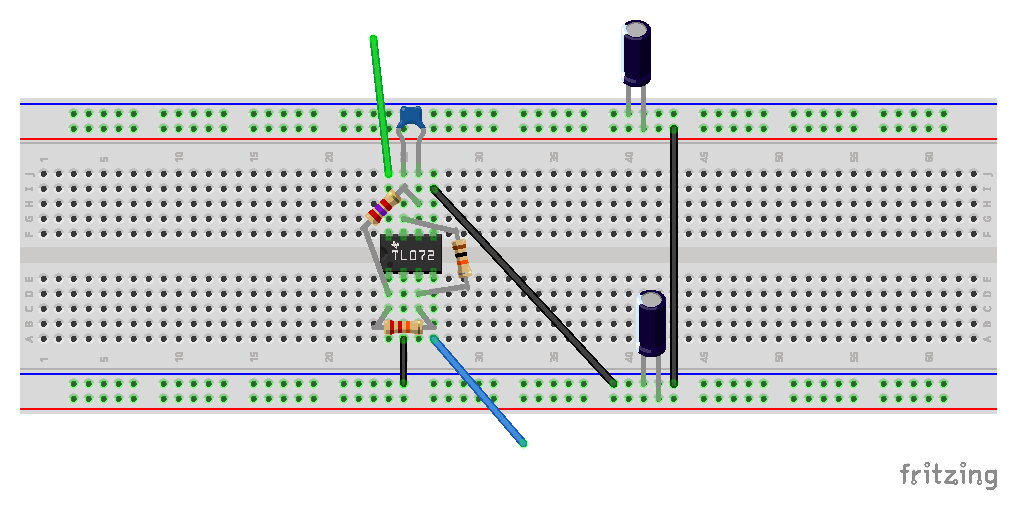
\includegraphics[width=0.5\linewidth]{Elektronik-Laborprotokoll_Filter/Abbildungen/Steckbrett_Bilder_Fritzing/Steckbrett_Dreieck_Rechteck.pdf}
  \caption{Dreieck-Rechteck-Oszillator (Steckbrett)}
  \label{fig:Steckbrett_Dreieck-Rechteck-Oszillator}
\end{figure}





%NE 555 Datenblatt

%1.Versuch
%********

%Wir benutzen 
%3 mal \SI{680}{\ohm} Widerstände
%3 mal \SI{100}{\nano\farad} Kondensatoren

%gelb ist Eingang
%rot ist Ausgang 

%Das Bodediagramm vom Hochpass aufgenommen mit einem Sinussignal mit der Amplitude 5 Volt

%als csv. 

%Vom Geräusch wurde 10Volt erzeugt, Magie

%120kOhm 
%120 Ohm  
%650Hz

%56kOhm   
%808Hz

%Das könnte man mit Potentiometer genau machen könnne.
%Im Idealfall sollte es eifentlich 29 sein,
%Da es Verkuste gibt, Caps, parasit¨ære Leckstrome usw. Es gibt ja Verluste
%Dann 29 reicht nicht aus.  

%2.Aufgabe
%1.Teil

%Mithilfe der Formel ..
%erhält man R=720 Ohm , haben wir aber 680

%NE555 wurde verwendet
% gebaut
%Kondensatoren imemr 100nF
%R1 berechnet 


%Versorgung war 12Volt

%Die Spannung Out Tri gemessen


%Dann misst man Tri (und Ground)
%transient


%Dann 3.Teil 
%die schaltung wurde von Fester 50\% duty cycle zu NE555 Monoflop umgewandelt
%Zeitkonstante war schon bestimmt: 1000


%5Volt VErsorgung

%Dann 2.Teil

%3.Aufgabe

%R wurde berechnet 


%K27.01.2024
%Kondensatoren 100nF, Widerstände nicht richtige

%wir haben E12